\chapter{Struttura causale}
Ad ogni punto $p$ dello spaziotempo, si associa un cono di luce, formato dalle geodetiche nulle emesse o assorbite dall'evento; nel cono si distinguono due regioni che nominiamo \emph{futuro} e \emph{passato}. Tutti gli eventi che giacciono all'interno del cono del futuro, rappresentano tutti quegli eventi che possono essere raggiunti da una particella massiva che parta da $p$, pertanto si dice che questi eventi costituiscano il futuro cronologico di $p$. Tutti gli eventi del futuro cronologico di $p$ e compresi quelli del cono del futuro, rappresentano gli eventi che possono essere in principio influenzati da $p$ e pertanto si parla di futuro causale di $p$.

In relatività generale la struttura causale dello spaziotempo è localmente della stessa natura dello spaziotempo piatto della relatività ristretta. Quando però si vengono a trattare topologie non banali, spazitempo singolari o quant'altro, emergono le differenze rispetto il caso noto.

Scopo di questa sezione è introdurre la descrizione della struttura globale dello spaziotempo facendo uso delle trasformazioni conformi e rappresentandola per mezzo dei \textbf{diagrammi di Penrose}. Come obiettivo finale c'è la descrizione rigorosa del concetto di buco nero.

I diagrammi di Penrose permettono di rappresentare questa struttura dopo che sia stata \textbf{compattificata} la topologia. Le varietà che sono state trattate sono varietà non compatte\footnote{Una varietà topologica si dice compatta se ogni suo ricoprimento aperto contiene un sottoricoprimento finito. Gli spazi illimitati (i.e. con diametro infinito o senza bordi) non possono essere compatti.}, compattificarle consiste nel portare l'infinito ad una distanza finita. Tale processo verrà effettuato volendo mantenere a 45 gradi i coni di luce.

\section{Definizioni formali della causalità}
\begin{definizione}
 Sia uno spaziotempo $(\mathcal{M},g)$ e un punto $x$ in esso. Il cono di luce $C_x$ è definito da quei vettori $v \in T_x\mathcal{M}$ tali che $-(v^0)^2 + \sum (v^i)^2 = 0$. Se è possibile definire un semicono futuro $C^+_x$ dato dai vettori $v_\mu v^\mu =0$, $v^0 \geq 0$ (\textit{future directed}) e un semicono passato $C^-_x$ dato dai vettori $v_\mu v^\mu = 0$, $v^0 \leq 0$ (\textit{past directed}), allora $T_x\mathcal{M}$ è \textbf{orientabile nel tempo.}

Se è possibile orientare nel tempo $T_x$  $\forall x \in \mathcal{M}$ in maniera continua, allora si dice che lo spaziotempo $\mathcal{M}$ è orientabile nel tempo.
\end{definizione}

Per quanto naturale come definizione, non è detto che tutti gli spazitempo possano essere orientabili nel tempo;  un esempio è lo spaziotempo ottenuto dai  punti $p, p'$  nel de Sitter mostrato in fig. \ref{fig.spazio_desitter}: questo spaziotempo è ottenuto dai punti identificati tramite riflessioni rispetto l'origine dello spazio di immersione. In questo spazio ci sono delle curve chiuse, non omotope a zero e per le quali l'orientamento del tempo è inverso. 

Quando uno spaziotempo $(\mathcal{M}, g)$ non è orientabile nel tempo, esiste uno spazio di doppio ricoprimento $(\tilde{\mathcal{M}},g)$ che lo è \cite{hawking}.

Consideriamo quindi spazitempo orientabili nel tempo. Possiamo far uso della divisione in future/past directed per definire:
\begin{definizione}
    Sia un punto $p \in \mathcal{M}$. Chiamiamo $I^+(p)$ \textbf{futuro cronologico} di $p$, l'insieme dei punti dello spaziotempo raggiungibili da $p$ con una curva di tipo tempo future directed.
    \begin{equation*}
        I^+(p)=\left\{ q \in \mathcal{M} | \exists C:[a,b]\rightarrow \mathcal{M}, C(a)= p, C(b)= q, \Dot{C}_\mu \Dot{C}^\mu < 0, \Dot{C}^0 >0 \right\}
    \end{equation*}
Definizione analoga per $I^-(p)$ \textbf{passato cronologico} di $p$, dove si richiede però che sia past directed.

Si definisce $J^+(p)$ \textbf{futuro causale} di $p$, l'insieme dei punti raggiungibili da $p$ con una curva non-tipo spazio ($\Dot{C}_\mu \Dot{C}^\mu \leq 0$) future directed. Analogo per $J^-(p)$ il \textbf{passato causale} di $p$.
\end{definizione}
Marginalmente, $I^+(\mathcal{S})$ rispetto un insieme $\mathcal{S}$, è un aperto poichè se un qualsiasi punto $q \in \mathcal{M}$ può essere raggiunto da una curva tipo tempo future directed da $\mathcal S$, allora esiste un intorno di $q$ che può essere raggiunto in tale modo.

\begin{definizione}
Definiamo:
\begin{itemize}
    \item $i_0$ l'infinito spaziale
    \item $i_\pm$, rispettivamente, l'infinito temporale futuro e passato
    \item $\mathcal{I}^\pm$, rispettivamente, l'infinito nullo futuro e passato
    \item $\mathcal{I} = \mathcal{I}^+ \cup \mathcal{I}^-$ l'infinito nullo
\end{itemize}
\end{definizione}

\begin{definizione}
Sia $p \in \mathcal{M}$. Si dice in $p$ vale la \textbf{causalità forte} se ogni intorno di $p$ contiene un intorno di $p$ che non viene intersecato più di una volta da ogni curva causale (non-\textit{spacelike}).
Lo spaziotempo è detto fortemente causale se la condizione vale $\forall p \in \mathcal{M}$.
\end{definizione}
Dunque se in un punto $p$ vale la causalità forte, non possono esistere curve causali che ritornano arbitrariamente vicino a $p$: in particolar modo non ci possono essere curve chiuse di tipo tempo o luce. Questa condizione permette di definire la \virgolette{forma} che possono avere le curve nello spaziotempo.

Sempre legata alla discussione della struttura causale dello spaziotempo, vi è il problema dei dati iniziali e di quali punti dello spaziotempo ne determino altri. Nella teoria newtoniana, dove le azioni a distanza sono istantanee, per predire eventi in punti futuri dello spaziotempo serve \virgolette{solamente} conoscere le condizioni dell'universo al tempo presente più alcune condizioni al bordo (come i potenziali che vanno a zero a infinito). Nella teoria relativistica, poiché differenti punti possono essere legati causalmente solo se possono essere connessi da curve non tipo spazio, la conoscenza dei dati di un determinato insieme $\mathcal{S}$ dello spaziotempo potrà determinare i soli eventi in una regione detta $D^+(\mathcal{S})$. Nel dettaglio:
\begin{definizione}
Definiamo $\Sigma$ una \textbf{superficie di Cauchy parziale} un'ipersuperficie di tipo spazio dello spaziotempo che non viene intersecata da alcuna curva causale più di una volta.
\end{definizione}
Possiamo quindi definire la regione prima anticipata:
\begin{definizione}
Si definisce il \textbf{future domain of dependence} $D^+(\Sigma)$ di $\Sigma$, l'insieme dei punti $p \in \mathcal{M}$ per i quali ogni curva causale inestensibile nel passato e che contiene $p$, interseca $\Sigma$.
\end{definizione}
II significato di $D^+(\Sigma)$ (e analogamente di $D^-(\Sigma)$) è che il comportamento delle soluzioni iperboliche alle equazioni alle derivate parziali date dalle equazioni di Einstein, al di fuori di $D^+$ non può essere determinato dai dati iniziali su $\Sigma$.  Il confine futuro di questa regione, formalmente $\overline{D^+(\Sigma)}\smallsetminus I^-(D^+(\Sigma))$, è \textbf{l'orizzonte di Cauchy futuro} di $\Sigma$. 
\begin{definizione}
Una superficie parziale di Cauchy $\Sigma$ è detta essere una \textbf{superficie di Cauchy} (globale) se vale:
\begin{equation*}
    D(\Sigma) := D^+(\Sigma) \cup D^-(\Sigma) = \mathcal{M}
\end{equation*}
Uno spaziotempo $\mathcal{M}$ che ha una superficie di Cauchy è detto \textbf{globalmente iperbolico}.
\end{definizione}
Si noti bene che la proprietà di un'ipersuperficie di essere di Cauchy non è propria della superficie, ma dello spaziotempo stesso nel quale è immersa. Se $\mathcal M$ non è globalmente iperbolica, allora $D^+(\Sigma)$ o $D^-(\Sigma)$ avranno un boundary in $\mathcal{M}$ che è proprio l'orizzonte di Cauchy futuro/passato.
\begin{figure}
    \centering
    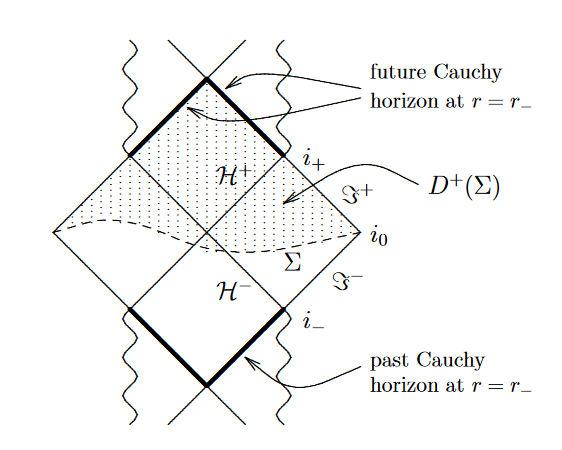
\includegraphics[scale=0.5]{immagini/cauchy_horizon.png}
    \caption{Esempio di superficie parziale di Cauchy, future domain of dependence e relativi orizzonti futuro/passato di Cauchy nella massima estensione analitica dello spaziotempo di Reissner-Nordstr\"om.}
    \label{fig.cauchy_horizon}
\end{figure}
Un esempio di superficie di Cauchy è l'ipersuperficie $t=\textrm{cost.}$ in Minkowski, mentre gli iperboloidi
\begin{equation*}
    t^2 - x^2 - y^2 - z^2 = \textrm{cost.}
\end{equation*}
sono ipersuperfici che giacciono interamente nel cono del passato dell'origine e sono solamente superfici parziali. O ancora se si considera lo spaziotempo di Minkowski privato di un punto, questo non può più ammettere superfici di Cauchy.

Con queste definizioni possiamo passare a trattare gli spazitempo utili alla descrizione dei buchi neri. Diversamente da quanto fatto per la cosmologia, dove l'interesse era quello di descrivere l'universo nella sua totalità e quindi era necessario introdurre un tensore energia-impulso che si estendesse per tutta la varietà, in questo caso ci soffermeremo su spazitempo che descrivono porzioni limitate dell'universo. L'interesse questa volta è descrivere come si comporta lo spaziotempo intorno ad una distribuzione limitata di materia, quindi per la descrizione di stelle e altri oggetti compatti. Il tensore energia-impulso sarà limitato ad una certa regione e non si estenderà all'infinito; la metrica descriverà le sole regioni esterne all'oggetto compatto. A tal fine sarà utile introdurre degli spazitempo che abbiano un comportamento semplice a distanze asintotiche.
\begin{definizione}
Uno spaziotempo orientabile nel tempo $(\mathcal{M}, g)$ è detto \textbf{asintoticamente semplice e vuoto} se esiste un embedding:
\begin{equation*}
    f: (\mathcal{M},g) \rightarrow (\Tilde{\mathcal{M}},g)\end{equation*}
che immerge $\mathcal{M}$  come varietà con bordo $\mathcal{I}$ nello spaziotempo fortemente causale $\Tilde{\mathcal{M}}$, tale che:
\begin{enumerate}
    \item Esiste una funzione differenziabile positiva $\Omega$ per cui
\begin{equation*}
    \Tilde{g}_{\mu\nu} = \Omega^2 g_{\mu\nu} \ \ \textrm{ in } \ \ \Tilde{\mathcal{M}}\cap \mathcal{M}
\end{equation*}
e vale che $\Omega = 0$ e $d\Omega \neq 0$ su $\mathcal{I}$.
\item Ogni geodetica nulla in $\mathcal{M}$ ha due estremi su $\mathcal{I}$.
\item $R_{\mu\nu}=0$ in un intorno aperto di $\mathcal{I}$ in $\Tilde{\mathcal{M}}$.
\end{enumerate}
Si scriverà $\mathcal{M}\cup \mathcal{I} = \Tilde{\mathcal{M}}$.
\end{definizione}
La prima richiesta corrisponde all'introdurre una metrica $\tilde{g}$ conforme alla metrica $g$ e più precisamente sono legate da $\Omega^2 g = f_*(\Tilde{g})$ con $f_*$ pull-back.
Le prime due richieste permettono di definire uno spaziotempo asintoticamente semplice, piuttosto generale e che include anche vari modelli cosmologici tra cui de Sitter. La terza richiesta fornisce il termine \virgolette{vuoto} e viene introdotta per restringerci ai soli spazi asintoticamente piatti.

La combinazione di $1.$ e $3.$ permette di mostrare che $\mathcal{I}$ è un'ipersuperficie nulla; il legame tra la curvatura scalare delle due metriche è ottenuto come riscalamento di Weyl \cite{wald}\cite{hawking} e ha la forma:
\begin{equation*}
    \Tilde{R} = \Omega^{-2}R - 6\Omega^{-1}\Omega_{|\mu\nu}\Tilde{g}^{\mu\nu} + 3\Omega^{-2}\Omega_{|\mu}\Omega_{|\nu}\Tilde{g}^{\mu\nu}
\end{equation*}
dove $|.$ indica la derivata covariante rispetto la metrica $\tilde{g}$. Supponendo $\Omega$ almeno di classe $\mathcal{C}^3$ su $\tilde{\mathcal{M}}$, allora $\tilde{g} \in \mathcal{C}^3$ e $\Tilde{R} \in \mathcal{C}^1$ sul bordo $\mathcal{I}$ dove $\Omega = 0$. Dunque $\Omega_{|\mu}\Omega_{|\nu}\Tilde{g}^{\mu\nu} = 0$ su $\mathcal{I}$ e poiché su questo bordo vale la condizione 1. $\Omega_{|\mu} \neq 0$, allora $\Omega_{|\nu}\Tilde{g}^{\mu\nu}$ dovrà essere un vettore nullo in quanto:
\begin{equation*}
    \Omega_{|\mu}\Tilde{g}^{\mu\nu}\Omega_{|\rho} \tilde{g}^{\rho\lambda} \Tilde{g}_{\nu\lambda} = \Omega_{|\mu}\Tilde{g}^{\mu\nu}\Omega_{|\rho}\tensor{\delta}{^\rho_\nu} = \Omega_{|\mu}\Omega_{|\rho}\Tilde{g}^{\mu\rho} = 0
\end{equation*}
dunque la ipersuperficie è nulla. Visto che $\mathcal{I}$ è una ipersuperficie nulla, si dovrà avere che $\mathcal{M}$  giaccia localmente nel passato e futuro di essa; per questo motivo $\mathcal{I}$ potrà avere soltanto due parti disconnesse $\mathcal{I}^-$ e $\mathcal{I}^+$ nelle quali si avranno gli estremi iniziali e finali delle geodetiche nulle in $\mathcal{M}$.

\'E importante notare che la richiesta $2.$ è particolarmente forte: spazi che sono asintoticamente semplici e vuoti sono, ad esempio, Minkowski e gli spazi asintoticamente piatti che descrivono oggetti legati che non vanno incontro a collasso gravitazionale; soluzioni che non rispettano la seconda condizione sono Schwarzschild, Reissner-Nordstr\"om e Kerr, per i quali esistono geodetiche nulle che non hanno \textit{endpoints} su $\mathcal{I}^+$ o $\mathcal{I}^-$. Tuttavia questi spazi hanno la caratteristica di essere asintoticamente piatti. Per questo motivo la seconda condizione viene modificata per introdurre lo spazio \textbf{debolmente asintoticamente semplice}:
\begin{enumerate}
\setcounter{enumi}{3}
\item Esiste un intorno aperto $U$ di $\mathcal{I}$ isometrico ad un intorno aperto di $\mathcal{I}'$ dello spazio asintoticamente semplice e vuoto $\mathcal{M}'$.
\end{enumerate}

\begin{teorema}
Se $\mathcal{M}$ è asintoticamente semplice e vuoto valgono:
\begin{enumerate}
    \item Ogni geodetica nulla in $\mathcal{M}$ che raggiunge $\mathcal{I}$ ha parametro affine illimitato ($\mathcal{I}^\pm$ è connessa con topologia $\mathbb{R}\times S^2$).
    \item $(\mathcal{M},g)$ è globalmente iperbolico
    \item $g$ approccia la metrica piatta di Minkowski, quindi è asintoticamente piatto.
\end{enumerate}
\end{teorema}
Le dimostrazioni possono essere trovate su \cite{hawking}. 

Per quanto riguarda il bordo $\mathcal{I}$, esso può essere pensato come all'infinito nel senso che, come detto dal teorema, qualsiasi geodetica nulla in $\mathcal{M}$ vi giunge con parametro affine illimitato. Detto $\lambda$ il parametro affine nella metrica $g$, esso è legato al parametro affine $\tilde{\lambda}$ di $\tilde{g}$ secondo:
\begin{equation*}
    \frac{d\lambda}{d\tilde{\lambda}}= \Omega^{-2}
\end{equation*}
Poiché $\Omega=0$ su $\mathcal{I}$, la quantità $\int d\lambda$ diverge e ciò spiega il primo punto del teorema. L'ultimo punto permette di dire che i diagrammi di Penrose per spazi asintoticamente semplici dovranno avere una forma condivisa con quella dello spazio di Minkowski.

\begin{definizione}
    Uno spaziotempo debolmente asintoticamente semplice e vuoto viene chiamato \textbf{asintoticamente predicibile nel futuro} se esiste una superficie di Cauchy parziale $\Sigma$ tale che:
\begin{equation*}
        \mathcal{I}^+ \subseteq \overline{D^+(\Sigma)}
\end{equation*}
dove con la barra si intende la chiusura nella varietà conforme $\tilde{\mathcal{M}}$.
\end{definizione}
Esempi di spazi che sono asintoticamente predicibili nel futuro a partire da una qualsiasi superficie $\Sigma$ sono Minkowski, Schwarzschild con $m\geq 0$, Kerr con $m\geq 0$, $m\geq |a|$ e Reissner.Nordstr\"om con $m\geq 0$, $m \geq |e|$.  La soluzione di Kerr con $m < |a|$ o Reissner-Nordstr\"om con $m < |e|$ non sono asintoticamente predicibili in quanto, per ogni superficie di Cauchy parziale $\Sigma$, ci sono curve inestensibili nel passato, di tipo tempo o nulle che partono da $\mathcal{I}^+$ e raggiungono la singolarità senza intersecare $\Sigma$. In altre parole la predicibilità asintotica del futuro può essere vista come quella condizione per la quale \textbf{non ci siano singolarità nude} nel futuro di $\Sigma$ ovvero singolarità che siano visibili da $\mathcal{I}^+$.

Possiamo infine definire il buco nero come la regione dello spaziotempo per la quale nessuna particella, massiva o massless, può fuggire verso l'infinito causale. La definizione formale è formulata \virgolette{al contrario}, andando a considerare tutti gli eventi di particelle che, nella loro evoluzione causale, hanno raggiunto l'infinito cronologico; il buco nero è quel che resta dello spaziotempo se si tolgono tutti i punti che hanno potuto raggiungere l'infinito:
\begin{definizione}
Lo spaziotempo $\mathcal{M}$ contiene un \textbf{buco nero} se
\begin{equation*}
    \mathcal{B}:= \mathcal{M}\smallsetminus J^-(\mathcal{I}^+) \neq \emptyset
\end{equation*}
La regione del buco nero viene chiamata $\mathcal{B}$, mentre il bordo di $J^-(\mathcal{I}^+)$ è detto $H$ orizzonte degli eventi.
\end{definizione}

Per chiarire ulteriormente questa definizione, in figura fig. \ref{fig.penrose_schwarz_buconero} sono evidenziate queste regioni.
\begin{figure}
    \centering
    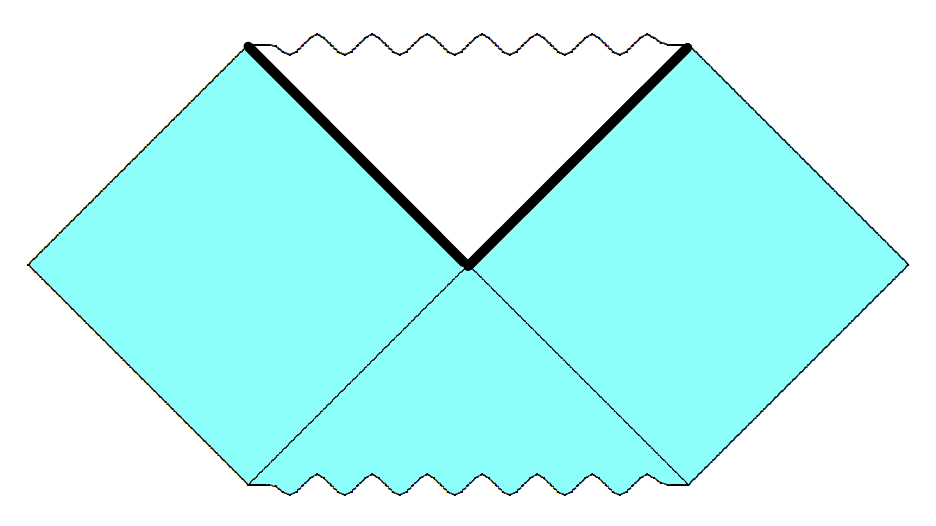
\includegraphics[scale=0.3]{immagini/schwarz_bh_regioni.png}
    \caption{In colore è mostrata la regione $J^-(\mathcal{I}^+)$, mentre quella lasciata in bianco corrisponde al buco nero. Il bordo evidenziato di nero è l'orizzonte degli eventi.}
    \label{fig.penrose_schwarz_buconero}
\end{figure}
\begin{figure}[t]
    \centering
    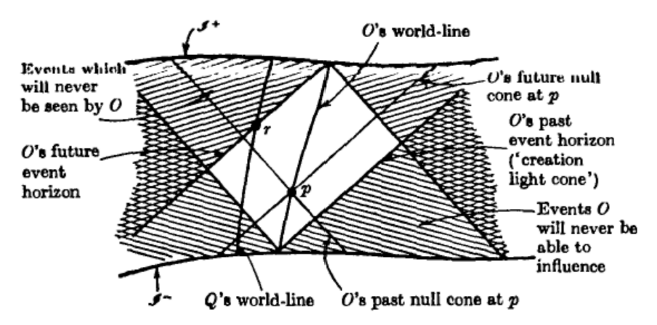
\includegraphics[scale=0.6]{immagini/horizons_hawk.png}
    \caption{Eventi che possono essere osservati o influenzati nella struttura causale di un generico spaziotempo.}
    \label{fig.orizzonti_hawk}
\end{figure}
\section{Causalità in Cosmologia}
In cosmologia risulta fondamentale introdurre nuovi tipi di orizzonti dello spaziotempo per studiare gli effetti causali tra diversi punti dell'Universo mentre questo si espande: date le dimensioni dell'Universo è importante capire quali eventi potranno essere da noi influenzati o diversamente a quali eventi noi abbiamo accesso tramite l'osservazione e quindi quale sia l'Universo osservabile. Legato a ciò vi è anche il cosiddetto \virgolette{problema dell'orizzonte} che insieme a quello della piattezza fa da apripista alla teoria dell'inflazione.

Consideriamo una famiglia di geodetiche tipo tempo, rappresentanti le linee di mondo di osservatori massivi; queste origineranno dall'infinito passato $\mathcal{I}^-$ e finiranno nell'infinito futuro $\mathcal{I}^+$. Chiamiamo $p$ un punto della geodetica di un osservatore $\mathcal{O}$: il cono nullo passato di $p$ è, come visto, il set di punti che possono essere osservati da $\mathcal{O}$ a quel tempo. Le linee di mondo di alcune particelle che intersecano questo cono nullo sono quelle viste da $\mathcal{O}$. In particolare ci sono quelle particelle le cui linee di mondo hanno origine in quei punti di $\mathcal{I}^-$ che sono intersecati dal cono passato di $\mathcal{O}$ e che delimitano un insieme di particelle che non potranno essere mai osservate da $\mathcal{O}$, fig. \ref{fig.particle_horizon_hawk}.
\begin{definizione}
La divisione di particelle che possono essere osservate da $\mathcal{O}$ in $p$ da quelle che non possono esserlo definisce l'\textbf{orizzonte delle particelle} per $\mathcal{O}$ in $p$.
\end{definizione}
\begin{figure}
    \centering
    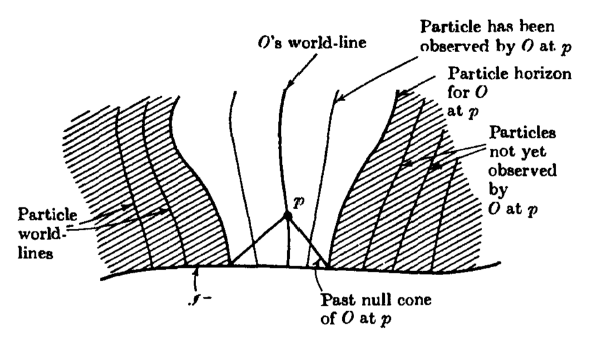
\includegraphics[scale=0.75]{immagini/particle_horizon_hawk.png}
    \caption{L'orizzonte delle particelle.}
    \label{fig.particle_horizon_hawk}
\end{figure}

L'esistenza del Big Bang impone che ci sia un tempo speciale che limita quanto indietro possiamo guardare nel passato. Indichiamo questo tempo con $t_{BB}$, ponendolo spesso a $0$. Nella cosmologia FLRW diventa:
\begin{definizione}
    L'\textbf{orizzonte delle particelle} (comovente) è la massima distanza (comovente) che ha potuto percorrere la luce dal Big Bang fino all'osservazione:
\begin{equation}
        r_{h}(t) = c\int_{t_{BB}}^t \frac{dt'}{a(t')}
        \label{eq.orizzonte_cosmologico_comovente}
\end{equation}
\end{definizione}
La distanza fisica corrispondente è data da $d_H = a(t)r_{h}(t)$ e corrisponde alle dimensioni dell'Universo osservabile. Nulla al di fuori di esso può influenzarci adesso. L'orizzonte dipende dal modello cosmologico adottato per $a(t)$ in eq. \ref{eq.friedmann_param_cosmologici}.  La definizione di orizzonte delle particelle può essere ugualmente parafrasata come \virgolette{la massima distanza con la quale ci può essere stato contatto causale dalla singolarità a una determinata epoca}.

\begin{definizione}
    L'\textbf{orizzonte degli eventi cosmologico} è la massima distanza comovente che la luce emessa ora può raggiungere un osservatore nel futuro.
    \begin{equation}
        r_{max}(t) = c \int_{t}^{t_{max}} \frac{dt'}{a(t')}
        \label{eq.event_horizon_comovente_cosmologia}
    \end{equation}
    dove $t_{max}$ è il tempo della fine dell'Universo, infinito se l'espansione non ha limite.
\end{definizione}
In altri termini, è la massima distanza che un oggetto può avere qualora venga osservato da un osservatore che osserva l'Universo al tempo $t$.
Si noti bene che l'orizzonte degli eventi cosmologico, a differenza di quello dei buchi neri, è dipendente dalla scelta dell'osservatore. 

Le proprietà degli orizzonti in cosmologia sono meglio studiate se si introduce una differente coordinata temporale.
\begin{definizione}
    Definiamo il \textbf{conformal time}:
    \begin{equation}
        \tau = \int^t_0 \frac{dt'}{a(t')} = \int_a^1 \frac{da}{a \Dot{a}} = \int_a^1\frac{da'}{a'^2 H(a')} = \int_z^0 \frac{(1+z')^2}{H(z')}dz'
        \label{eq.conformal_time}
    \end{equation}
\end{definizione}
Solitamente il conformal time è segnato con $\eta$. Di fatto è la distanza comovente divisa per la velocità della luce $c$. \'E monotona crescente e per questo motivo può essere usata come variabile temporale.
Questa coordinata permette di riscrivere la metrica FLRW, eq. \ref{eq.metrica_flrw} nella forma\footnote{Qui $\chi$ è la coordinata spaziale comovente che può essere adimensionale o dimensionata a seconda delle convenzioni, pertanto in altri luoghi potrebbe essere moltiplicata per una scala $R$ che fornisce la dimensione di lunghezza. In questo caso omettiamo la dimensione così come mettiamo $c=1$.}:
\begin{equation}
    ds^2 = a(t)^2\left[ - d\tau^2 + d\chi^2 + S_k^2(\chi)(d\theta^2 + \sin^2\theta d\phi^2)\right]
    \label{eq.metrica_flrw_conformal_time}
\end{equation}
In questo modo le curve luce sono, in un piano $(\tau, \chi)$,  delle linee a 45°. L'orizzonte delle particelle e quello cosmologico possono essere raffigurati come in fig. \ref{fig.particle_horizon_conforme}-\ref{fig.orizzonte_cosmologico_conforme}. Con questa definizione di tempo, l'orizzonte delle particelle è semplicemente:
\begin{equation*}
    r_{h} = c(\tau - \tau_{BB})
\end{equation*}
Viene altrettanto usato definire $c(aH)^{-1}$  come il \textbf{comoving Hubble radius}, mentre il raggio di Hubble proprio è solamente $cH^{-1}$. Solitamente ci si riferisce a quest'ultimo come \virgolette{l'orizzonte} in quanto fornisce una stima della distanza che la luce può percorrere mentre l'Universo si espande in una maniera apprezzabile, quindi permette di descrivere le dimensioni di regioni di Universo che sono tra loro in contatto causale. Si noti bene che rispetto l'orizzonte di particelle, il raggio di Hubble definisce la distanza di contatto causale \emph{ad una determinata} epoca, quindi risulta più utile per descrivere il contatto causale con l'evoluzione dell'Universo. Quando una determinata scala esce dall'orizzonte, si interrompe il contatto causale e si ha il \textbf{freeze out} finché non vi rientrerà.

Il comoving Hubble radius può ulteriormente essere confuso con l'orizzonte delle particelle se riscriviamo l'orizzonte delle particelle comovente di prima (ovvero il conformal time con $c=1$):
\begin{equation*}
    r_h = c \int_{t_{BB}}^t\frac{dt'}{a(t')} = \int_{\log a_{BB}}^{\log a} c(a'H)^{-1}d\log a'
\end{equation*}
Per le sorgenti di materia ordinaria, il raggio di Hubble comovente è monotono crescente col tempo e il contributo dell'integrale qui sopra è dominato nei \textit{late times}, permettendo nella cosmologia standard $r_h \sim c(aH)^{-1}$.
\begin{figure}
    \centering
    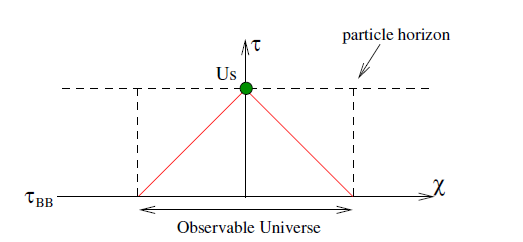
\includegraphics[scale=0.8]{immagini/particle_horizon_conforme.png}
    \caption{L'orizzonte delle particelle nel tempo conforme.}
    \label{fig.particle_horizon_conforme}
\end{figure}
\begin{figure}
    \centering
    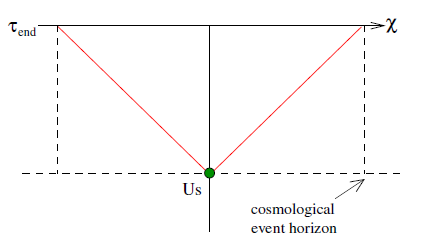
\includegraphics[scale=0.7]{immagini/orizzonte_cosmologico.png}
    \caption{L'orizzonte cosmologico nel tempo conforme}
    \label{fig.orizzonte_cosmologico_conforme}
\end{figure}
\begin{esempio}
In un Universo Einstein-de Sitter $(\Omega_0 = 1, \Omega_\Lambda =0 )$ il fattore di scala determinato dall'eq. di Friedmann, eq. \ref{eq.friedmann_param_cosmologici} evolve col tempo cosmico come $a \propto t^{2/3}$. Di conseguenza l'orizzonte di particelle comovente e proprio sono rispettivamente $r_{H,com} =3 t^{1/3} $, $r_H = 3t$, mentre il raggio di Hubble $r_{HS, com} = \frac{3}{2}t^{1/3}$, $r_{HS} = \frac{3}{2}t$ . Non esiste l'orizzonte degli eventi per questo modello. Chiamando $t_0 = \frac{2}{3}$, il tempo conforme è $\tau = 2(t/t_0)^{1/3}$ così che le precedenti comoventi diventano: $r_{H,com} = \tau$, $r_{HS, com} = \frac{\tau}{2}$.
\end{esempio}
\begin{figure}
    \centering
    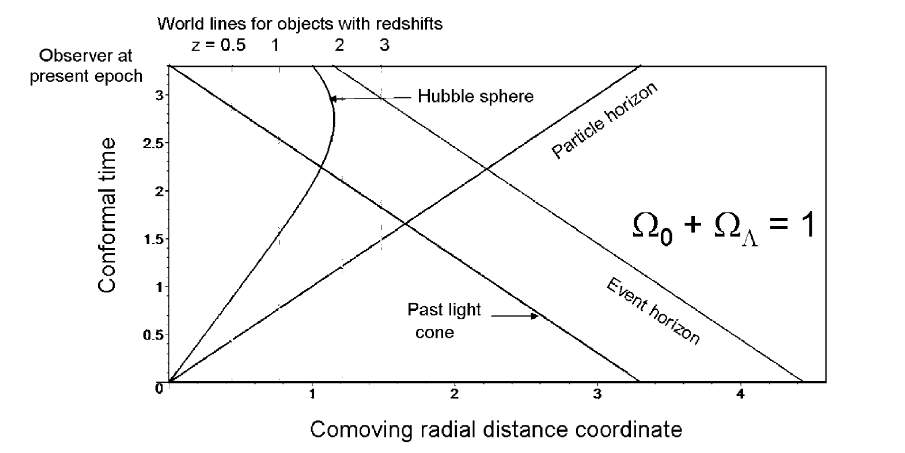
\includegraphics[scale=0.4]{immagini/lcdm_causaleconforme.png}
    \caption{Orizzonte di particelle, cono luce, orizzonte degli eventi e sfera di Hubble  in coordinate e tempo comoventi per la cosmologia standard $\Omega_0 = 0.3, \Omega_\Lambda = 0.7$. Orizzonte degli eventi e raggio di Hubble tendono a zero per $t\rightarrow \infty$: l'espansione accelerata porta le galassie a distanze dove non ci può più essere contatto causale con l'osservatore all'epoca $t$.}
    \label{fig.lcdm_causale}
\end{figure}
\section{Diagrammi di Penrose}
\subsection{Spazio Euclideo 2d}
Spieghiamo il procedimento direttamente considerando il caso semplice di $\mathbb{E}^2$.

La metrica dello spazio è:
\begin{equation*}
    ds^2 = dx^2 + dy^2 = dr^2 + r^2d\phi^2
\end{equation*}
Tale spazio risulta banale, visto che non è presente alcuna \emph{timeline}, quindi non possiede causalità. Tuttavia è istruttivo per gli esempi successivi.

L'idea per compattificare tale spazio, è quella di introdurre un cambio di coordinate del tipo $r= f(\theta)$ tale che per $r\rightarrow + \infty$ si abbia $\theta$ finito. Tra le funzioni che divergono per valori finiti, scegliamo la tangente. Questa risulterà particolarmente utile negli esempi successivi.
\begin{equation*}
    r = \tan\frac{\theta}{2} \implies dr= \frac{d\theta}{2\cos^2\frac{\theta}{2}}
\end{equation*}
così che la metrica diventa:
\begin{equation*}
    ds^2 =\frac{1}{4\cos^4\frac{\theta}{2}}[ d\theta^2 + \sin^2\theta d\phi^2]
\end{equation*}
Il prefattore diverge pertanto effettuiamo una trasformazione conforme della metrica:
\begin{equation*}
    d\tilde{s}^2 = 4\cos^4\frac{\theta}{2} ds^2 = d\theta^2 + \sin^2\theta d\phi^2
\end{equation*}
In questo modo tutti i punti di $\mathbb{E}^2$ sono stati portati sulla 2-sfera unitaria: si dice che $\mathbb{E}^2$ è conforme a $S^2$. Di fatto stiamo definendo una metrica
\begin{equation*}
    \tilde{g}_{\mu\nu}(x) = \Omega^2(x)g_{\mu\nu}
\end{equation*}
differente dall'iniziale, ma che preserva la struttura causale. 
\subsection{Spazio di Minkowski (1+1)d}
La metrica è:
\begin{equation*}
    ds^2 = -dt^2 + dx^2
\end{equation*}
con $t, x \in (-\infty,+\infty)$. Anticipiamo ora, ma lo vedremo in dettaglio nell'esempio successivo, che la compattificazione che si ottiene per lo spazio di Minkowski $(1+1)d$ è differente da quella di Minkowski $(1+3)d$ in quanto in quest'ultima, sfruttando la simmetria delle coordinate sferiche, le due variabili che dovremo trattare saranno $t, r$ dove $r \in (0,+\infty)$.

Tornando al presente caso, le strutture di interesse all'interno di Minkowski $(1+1)d$ sono rappresentate dalle rette luce $t\pm x = \textrm{cost.}$, nonché dalle rette verticali $x = \textrm{cost.}$ (rappresentanti un punto fisso spazialmente) e orizzontali $t = \textrm{cost.}$, del piano di Minkowski.

Facciamo quindi il cambio di coordinate, prendendo le outgoing e ingoing, rispettivamente:
\begin{align*}
    u = t - x && v = t + x
\end{align*}
con $u, v \in (-\infty,+\infty)$. La metrica diventa:
\begin{equation*}
    ds^2 = - dudv
\end{equation*}
Effettuiamo la compattificazione:
\begin{align*}
     u = \tan \tilde{u} && v = \tan \tilde{v}
\end{align*}
per ottenere la metrica:
\begin{equation*}
    ds^2 = - \frac{1}{\cos^2\tilde{u}\sin^2\tilde{v}}d\tilde{u}d\tilde{v}
\end{equation*}
Passando alla metrica conforme:
\begin{equation*}
    d\tilde{s}^2 = \cos^2\tilde{u}\sin^2\tilde{v} ds^2 = - d\tilde{u}d\tilde{v}
\end{equation*}

Abbiamo così compattificato lo spazio di Minkowski bidim. nelle variabili $\tilde{u}$, $\tilde{v}$, ottenendo una metrica $d\tilde{s}^2$ finita su tutto lo spazio e che preserva la struttura causale. Eseguiamo l'ultimo cambio di variabili:
\begin{align*}
\left\{\begin{array}{l}
    T = \frac{\tilde{u}+\tilde{v}}{2} \\ \\
    X = \frac{\tilde{v}-\tilde{u}}{2}
\end{array}\right.
\implies d\tilde{s}^2 =-dT^2 + dX^2
\end{align*}
dove però $T, X \in ( -\frac{\pi}{2}, \frac{\pi}{2})$. Il diagramma di Penrose, fig. \ref{fig.pen_mink_11}, è la rappresentazione grafica di tale spazio. Di fatto abbiamo potuto rappresentare tutto lo spazio di Minkowski all'interno di questo grafico. Potendo scrivere:
\begin{align*}
    t - x = \tan(T-X) && t + x = \tan(T+X) 
\end{align*}
si ottengono facilmente:
\begin{align*}
    x = \frac{1}{2}\left[ \tan(T+X) - \tan(T-X)\right] && t = \frac{1}{2}\left[ \tan(T+X) + \tan(T-X)\right]
\end{align*}
\begin{figure}
    \centering
    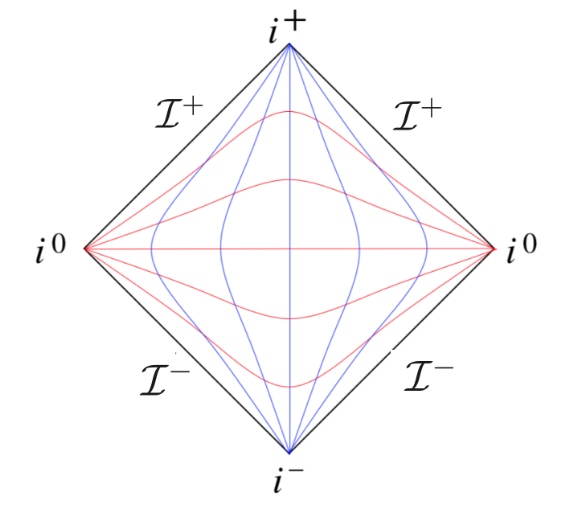
\includegraphics[scale=0.58]{immagini/penrose_mink_11.png}
    \caption{Diagramma di Penrose dello spazio Minkowski $(1+1)d$.}
    \label{fig.pen_mink_11}
\end{figure}

Nella figura sono rappresentate in blu le rette $x = \textrm{cost.}$ e in rosso $t = \textrm{cost.}$ che sono state mappate tramite la conformazione conforme nel diagramma secondo le relazioni calcolate qui sopra.

Si osserva che tutti i moti in blu nascono da un punto all'infinito $i^-$ (\emph{i minus}) detto \textbf{infinito del passato} e giungono in un tempo infinito nello stesso punto $i^+$ (\emph{i plus}) detto \textbf{infinito del futuro}. Questi sono punti di tipo tempo. La compattificazione ha proprio lo scopo di rappresentare finitamente questi infiniti che altrimenti sul piano di Minkowski non sarebbero visibili. Le curve in rosso invece originano e giungono nello stesso punto $i^0$ detto \textbf{infinito di tipo spazio}. Alcune volte si distingue in $i_L$ e $i_R$, ma sono in realtà lo stesso punto per la simmetria.

Le curve di tipo luce $t \pm x = \textrm{cost.}$ rimangono rette di 45 gradi a formare una griglia nel diagramma. Queste originano dai due lati obliqui inferiori $\mathcal{I}^-$ (\emph{scri minus}) e finisco in quelli superiori $\mathcal{I}^+$ (\emph{scri plus}). Aspetto fondamentale è che le particelle originano e finiscono tutte negli stessi punti, indipendentemente dal tipo di geodetica seguita; la luce invece ha origine per ogni punto di $\mathcal{I}^-$. In coordinate $\mathcal{I}^- = ( -\frac{\pi}{2}, \cdot)$ e $\mathcal{I}^+ =( \cdot, \frac{\pi}{2})$.

Osserviamo che si ritrova il fatto che nessuna particella massiva, che segue le curve in blu, può andare più veloce della luce in quanto qualunque sia la geodetica seguita, la tangente avrà sempre un angolo minore di 45 gradi.

Altre importanti osservazioni. Per prima cosa si ha che ogni osservatore, asintoticamente, vede tutto lo spazio nel suo passato. Questo può essere notato considerando le rette luce orientate \virgolette{verso il basso} che possono essere originate da ogni punto lungo le curve blu: stiamo parlando del cono di luce del passato. Risulta quindi evidente che quando l'osservatore si trova in $i^+$, le sue rette luce del passato coincideranno con $\mathcal{I}^+$ e quindi il suo cono del passato coinciderà con tutto lo spazio.
Per seconda cosa, qualsiasi coppia di eventi sono connessi causalmente nel passato e si possono influenzare nel futuro. Infatti se si rappresenta il cono di luce passato e futuro per ognuno dei due punti, inevitabilmente si avrà una regione di intersezione nel passato e una nel futuro. Questo aspetto è fondamentale in ambito cosmologico in quanto si ha accesso solo ad uno spazio finito e pertanto, a livello globale, il nostro universo non può essere di Minkowski.

\subsection{Spazio di Minkowski (1+3)d}
La metrica:
\begin{equation*}
    ds^2= -dt^2 + dx^2 + dy^2 + dz^2 = -dt^2 + dr^2 + r^2d\Omega_2^2
\end{equation*}
dove con $d\Omega_2$ rappresenta la 2-sfera. Applichiamo ancora il cambio di coordinate outgoing, ingoing: $u = t - r$, $v = t+ r$ per avere:
\begin{equation*}
    ds^2 =-dudv + \frac{(u-v)^2}{4}d\Omega_2^2
\end{equation*}
Compattificando con $u = \tan\tilde{u}$, $v = \tan\tilde{v}$, si ottiene:
\begin{equation*}
    ds^2 = \frac{1}{4\cos^2\tilde{u}\sin^2\tilde{v}}\left[ - d\tilde{u}d\tilde{v} + \sin^2(\tilde{v}-\tilde{u})d\Omega_2^2\right]
\end{equation*}
con $\tilde{u}, \tilde{v} \in (-\frac{\pi}{2}, \frac{\pi}{2})$. Definiamo quindi la metrica conforme:
\begin{equation*}
    d\tilde{s}^2 = - 4 d\tilde{u}d\tilde{v} + \sin^2(\tilde{v}-\tilde{u})d\Omega_2^2
\end{equation*}
Poiché $r>0$ e $r = \frac{1}{2}(v-u)$ si avrà necessariamente $v > u$ ovvero $\tilde{v} > \tilde{u}$. Ciò comporta che il diagramma non avrà la stessa forma a diamante del caso $(1+1)d$.

Definendo anche qui:
\begin{align*}
    T = \tilde{u} + \tilde{v} && R = \tilde{v} - \tilde{u}
\end{align*}
si ottiene la metrica:
\begin{equation*}
    d\tilde{s}^2 = - dT^2 + dR^2 +\sin^2R d\Omega_2^2
\end{equation*}
Si osserva che il termine $\sin^2R d\Omega_2^2$ rappresenta una 3-sfera, da pensare come una sfera con raggio che varia con lo stesso $R$. Per questioni di simmetria, nel diagramma si sopprimerà questa parte di coordinate.
Il legame con le coordinate iniziali:
\begin{align*}
    t - r= \tan\left( \frac{T - R}{2}\right) &&  t + r = \tan\left( \frac{T + R}{2}\right)
\end{align*}
con $|T| + R \leq \pi $. Il diagramma di Penrose per Minkowski $(1+3)d$ è mostrato in fig. \ref{fig.pen_mink_13}.
\begin{figure}
    \centering
    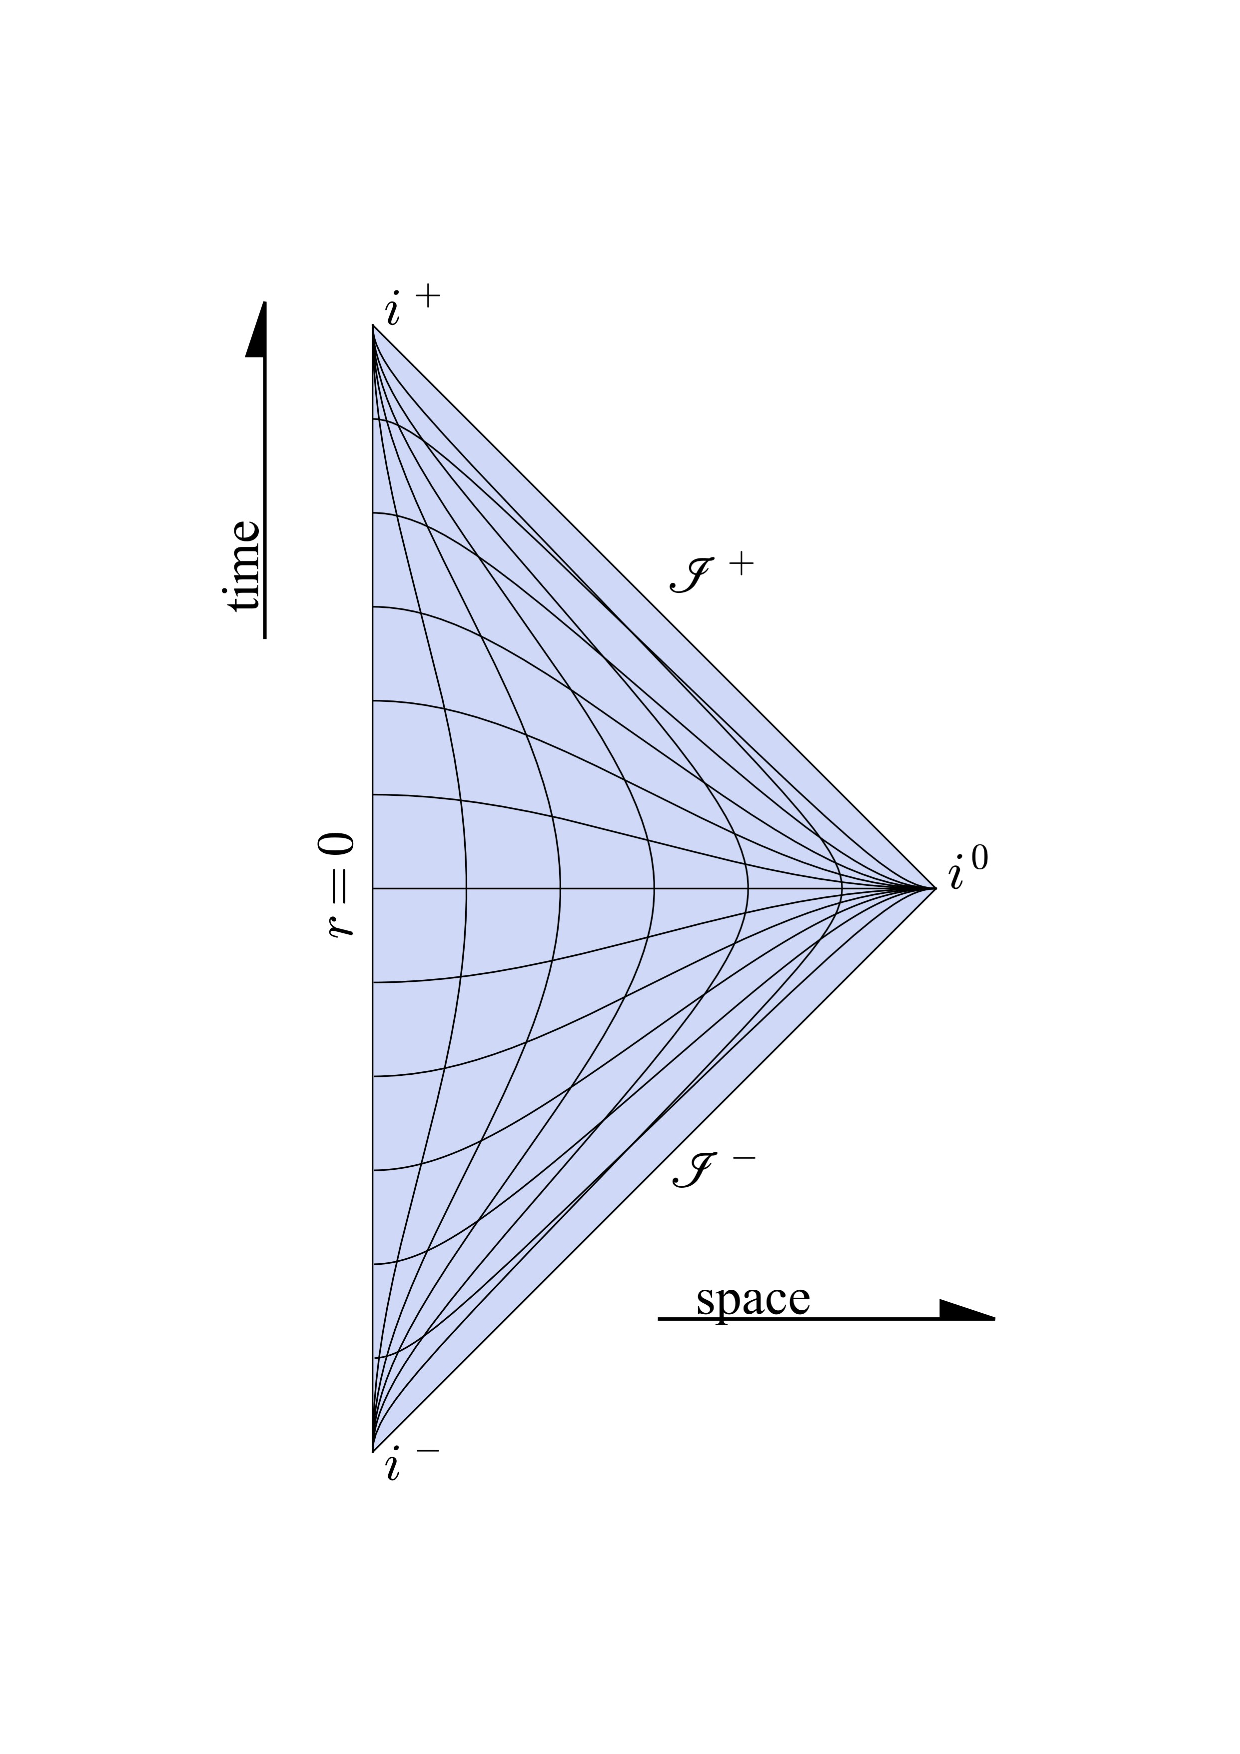
\includegraphics[scale=0.35]{immagini/mink4d.pdf}
    \caption{Il diagramma di Penrose per Minkowski $(1+3)d$.}
    \label{fig.pen_mink_13}
\end{figure}

Tale diagramma è caratterizzato da solo metà diamante per via della restrizione iniziale $r>0$ che differiva dalla richiesta iniziale $x\in\mathbb{R}$ del caso bidimensionale; tutto il bordo verticale di sinistra, corrispondente a $r=0$, non è infatti un contorno dello spazio, ma è dovuto solo a questa richiesta. Nonostante ciò sono presenti gli stessi punti di infinito $i^-$, $i^+$, $i^0$, origine e fine delle geodetiche tipo luce, spazio e $\mathcal{I}^-$, $\mathcal{I}^+$ come origine delle geodetiche nulle. Le curve relative a $t= \textrm{cost.}$ sono ottenute da:
\begin{equation*}
    t= \frac{1}{2}\left[  \tan\left( \frac{T + R}{2}\right)  -  \tan\left( \frac{T - R}{2}\right)\right]
\end{equation*}

Per lo spazio Minkowski $(1+3)d$ valgono le stesse osservazioni del caso bidimensionale, in particolare quelle esposte alla fine del precedente esempio, riguardo la possibilità di osservare tutto lo spazio in un tempo sufficientemente grande e che due qualsiasi eventi sono causalmente connessi nel passato e futuro.

\subsection{Spazio di de Sitter}
La metrica dello spazio di de Sitter statico, \S\ref{para.desitterstatici}, è:
\begin{equation*}
    ds^2 = - \left( 1 - \frac{r^2}{R^2} \right)dt^2 + \left( 1 - \frac{r^2}{R^2} \right)^{-1}dr^2 + r^2(d\theta^2 + \sin^2\theta d\phi^2)
\end{equation*}

Se effettuiamo l'embedding nello spazio di Minkowski 5-dim. di metrica:
\begin{equation*}
    ds^2 = -(dX^0)^2 + \sum_{i=1}^4 (dX^i)^2
\end{equation*}
ed effettuiamo il cambio di coordinate:
\begin{align*}
    X^0=R\sinh(\tau/R) && X^i = R\cosh(\tau/R)y^i \quad \textrm{dove} \quad \sum_{i=1}^4 (y^i)^2 = 1
\end{align*}
(questi ultimi parametrizzano la 3-sfera) si ottiene la metrica per lo spazio di de Sitter:
\begin{equation*}
    ds^2 = -d\tau^2 + R^2\cosh^2(\tau/R)d\Omega_3^2
\end{equation*}

Si definisce il \textbf{conformal time}:
\begin{equation*}
    \frac{d \eta}{d\tau} = \frac{1}{R\cosh(\tau/R)}
\end{equation*}
affinché si possa passare da $\tau \in (-\infty,+\infty)$ ad un nuovo tempo $\eta$ che sia invece finito. In particolare risolvendo si ottiene:
\begin{equation*}
    \cos \eta = \frac{1}{\cosh(\tau/R)}
\end{equation*}
così che $\eta \in (- \frac{\pi}{2}, \frac{\pi}{2})$. Facendo questo cambio di coordinate nella metrica:
\begin{equation*}
    ds^2 = \frac{R^2}{\cosh^2\eta}\left[ - d\eta^2 + d\Omega_3^2 \right] = \frac{R^2}{\cosh^2\eta}\left[ - d\eta^2 + d\chi^2 + \sin^2\chi d\Omega_2^2\right]
\end{equation*}
con $\chi \in (0,\pi)$. Risulta conformemente equivalente alla metrica:
\begin{equation*}
    d\tilde{s}^2 = - d\eta^2 + d\chi^2 + \sin^2\chi d\Omega_2^2
\end{equation*}
Omettendo la parte di simmetrica sferica, si ottiene il diagramma di Penrose di fig. \ref{fig.pen_desitter}. Tale spazio è un quadrato nel quale i punti $i^+, \mathcal{I}^+$ e $i^-, \mathcal{I}^-$ coincidono, quindi le geodetiche di tipo tempo e luce hanno stessa origine e termine. \'E importante notare che le linee verticali laterali non sono \emph{boundaries} dello spazio, ma semplicemente corrispondono ai polo nord e sud della 3-sfera. I veri limiti infiniti che sono stati compattificati sono i lati orizzontali.

A differenza dello spazio di Minkowski, non è vero che un qualsiasi osservatore, aspettando un tempo sufficiente, possa vedere tutto lo spazio. Un osservatore posto nel vertice in alto a sinistra possiede un cono del passato che riempe tutta la diagonale inferiore del quadrato e pertanto è capace di vedere solo metà dello spaziotempo; la diagonale che delimita le due regioni è l'\textbf{orizzonte degli eventi}: al di fuori di essa gli eventi non possono essere influenzati da ciò che si trova dentro.
Viceversa un osservatore posto nel vertice in basso a sinistra possiede un cono del futuro che gli permette di interagire solo con l'altra semi-regione dello spaziotempo; la diagonale delimitante viene detta \textbf{orizzonte delle particelle}: le particelle massive non possono raggiungere tutto lo spazio in un tempo finito.

Da un punto di vista cosmologico si è visto che l'attuale universo ha le caratteristiche di uno spazio di de Sitter, pertanto ci sono parti dell'universo alle quali non avremo mai accesso.
\begin{figure}
    \centering
    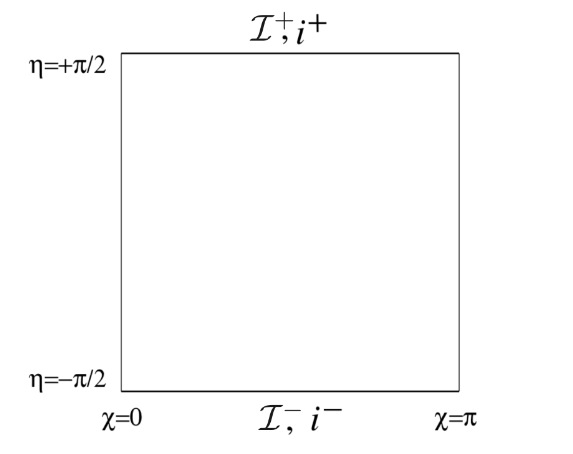
\includegraphics[scale=0.6]{immagini/desitter_penrose.png}
    \caption{Il diagramma di Penrose per lo spazio di de Sitter.}
    \label{fig.pen_desitter}
\end{figure}
\subsection{Soluzione di Schwarschild}
Il procedimento effettuato in \S\ref{para.kruskal} ha permesso di ottenere nuove importanti caratteristiche della soluzione di Schwarzschild ed in particolare, attraverso le coordinate di Kruskal-Szekeres, ci ha permesso di scrivere la metrica:
\begin{equation*}
    ds^2 = -\frac{32M^3e^{-r/2M}}{r}dUdV + r^2(U,V)d\Omega_2^2
\end{equation*}
dove si hanno giustamente i coni luce a 45 gradi, ma manca la compattificazione. Definendo come solito:
\begin{align*}
    U=\tan\tilde{U} && V = \tan\tilde{V}
\end{align*}
si ottiene:
\begin{equation*}
    ds^2 = \frac{1}{\cos^2\tilde{U}\cos^2\tilde{V}} \left[  -\frac{32M^3 e^{-r/2M}}{r}d\tilde{U}d\tilde{V} + r^2\cos^2\tilde{U}\cos^2\tilde{V}d\Omega_2^2\right]
\end{equation*}
Quindi rimuovendo il fattore conforme:
\begin{equation*}
    d\tilde{s}^2 =  -\frac{32M^3 e^{-r/2M}}{r}d\tilde{U}d\tilde{V} + r^2\cos^2\tilde{U}\cos^2\tilde{V}d\Omega_2^2
\end{equation*}

Vediamo i punti e le regioni di rilevanza per la struttura causale nelle nuove coordinate:
\begin{itemize}
    \item $r = 0$ corrisponde in coordinate di Kruskal $UV=1$ che nelle coordinate conformi:
    \begin{equation*}
        \tan\tilde{U}\tan\tilde{V} = 1 \iff \sin\tilde{U}\sin\tilde{V}-\cos\tilde{U}\cos\tilde{V}=0 \iff \cos(\tilde{U}+\tilde{V})=0
    \end{equation*}
    ovvero $\tilde{U}+\tilde{V}= \pm \frac{\pi}{2}$.
    \item $r=2M$ corrisponde a $U , V = 0$ ovvero semplicemente $\tilde{U}, \tilde{V}=0$.
    \item $r>2M$ ovvero $U, V > 0$ e cioè $\tilde{U}, \tilde{V}>0$.
\end{itemize}
Osserviamo che la scelta della tangente per compattificare, permette si semplificare molto questi calcoli. In maniera analoga si possono definire le quantità:
\begin{align*}
    T = \tilde{U}+ \tilde{V} && R = \tilde{V}- \tilde{U}
\end{align*}
da non confondere con le $T, R$ basate sulle coordinate di Kruskal. In fig. \ref{fig.penrose_schwarz} è rappresentato il diagramma della soluzione estesa di Schwarzschild (gli assi $\tilde{U},\tilde{V}$ sono ruotati in 45 gradi e corrispondono come visto sopra alle rette $r=2M$); sono anche rappresentate le quattro regioni già trattate in \S\ref{para.kruskal} corrispondenti al nostro universo (I), il buco nero (II), l'altro universo (III) e il buco bianco (IV).
\begin{figure}
    \centering
    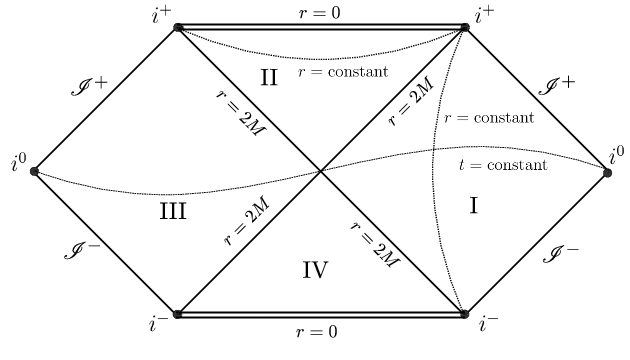
\includegraphics[scale=0.65]{immagini/penrose_schwarz.png}
    \caption{Il diagramma di Penrose della soluzione estesa di Schwarzschild.}
    \label{fig.penrose_schwarz}
\end{figure}

Limitandoci per il momento a discutere il quadrato di destra, tornano i punti di infinito $i^-$, $i^+$ per le particelle e i $\mathcal{I^-}$, $\mathcal{I}^+$ per la luce. I due bordi di sinistra corrispondono invece all'orizzonte del passato $H^-$ e l'orizzonte degli eventi $H^+$. Possiamo osservare che la metà di destra di tale quadrato condivide la stessa struttura causale dello spazio di Minkowski $(1+3)d$ e questo è dovuto al fatto che la soluzione di Schwarzschild è asintoticamente piatta. Le geodetiche che originano in $i^-$ e finiscono nell'orizzonte $H^+$ sono quelle destinate a finire nel buco nero, non potendo uscire in quanto servirebbe un'inclinazione superiore a 45 gradi.

La geodetica $t=\textrm{cost.}$ rappresentata e passante per l'origine del grafico, è il tipo di geodetica che permette di collegare i due universi (l'origine è il ponte di Einstein-Rosen già visto) che chiaramente non è percorribile in quanto implicherebbe $v>c$.

Consideriamo la geodetica di una particella che finisce nel buco nero; eventualmente consideriamo che la sua velocità sia particolarmente relativistica, linea rossa in fig. \ref{fig.penschwarz_orizz}. Immaginiamo che questo osservatore massivo emetta dei fotoni, rappresentate dalle rette luce in blu, e che questi vengano ricevuti da un altro osservatore fisso a $r = \textrm{cost.}$, in arancione.
Innanzitutto si può osservare che per tempi infinitamente lontani, si potrebbe credere che il segnale inviato dall'osservatore rosso sia invece partito dal buco bianco. L'aspetto invece fondamentale è che più l'osservatore in rosso si avvicina all'orizzonte, più sarà il tempo richiesto affinché il segnale giunga all'osservatore arancione. Al limite, quando vi si troverà all'orizzonte $H^+$, il segnale luminoso potrà giungere all'osservatore arancione solo quando esso si troverà nel suo punto di infinito $i^+$.
In altri termini, serve un tempo infinito per poter mappare tutto lo spaziotempo e poter definire l'orizzonte. Questo porta alla conclusione che \textbf{l'orizzonte degli eventi non è locale} in quanto esso è definito come il \emph{boundary} a infinito del cono del passato di una geodetica di tipo tempo (ad esempio la arancione della figura).
\begin{figure}
    \centering
    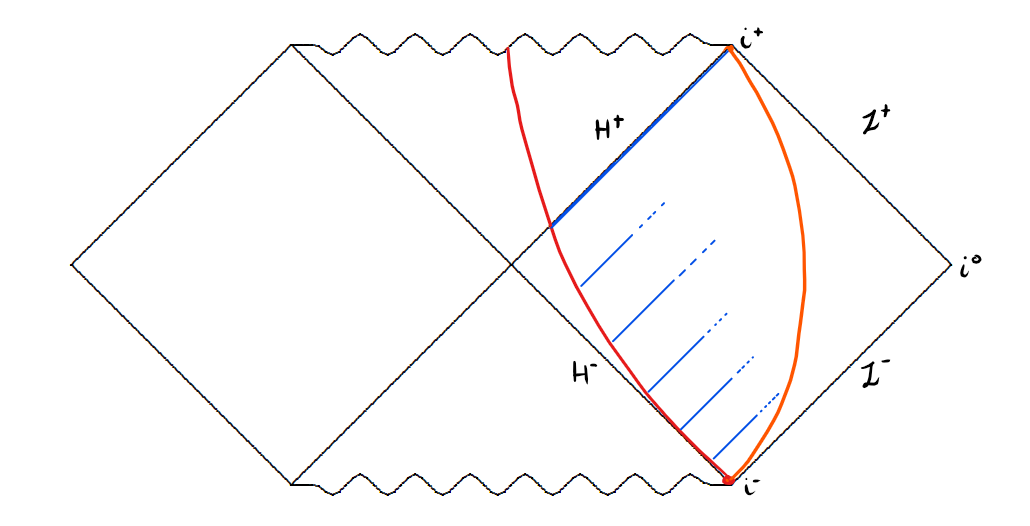
\includegraphics[scale=0.45]{immagini/penschwarz_orizz.png}
    \caption{Particella relativistica (linea rossa) che finisce nella singolarità, mentre emette fotoni (linee blu) ricevuti dall'osservatore a $r=\textrm{cost.}$ (linea arancione). Più si avvicina all'orizzonte degli eventi, più verrà richiesto un tempo al limite infinito per ricevere il segnale.}
    \label{fig.penschwarz_orizz}
\end{figure}
\subsection{Singolarità nuda in Schwarzschild}
La soluzione di Schwarzschild presenta una singolarità nuda, cioè che può essere vista a $\mathcal{I}^+$ quando $M<0$; dal punto di vista fisico ciò non ha senso, ma la soluzione soddisfa comunque le equazioni di Einstein e pertanto vale la pena analizzarla.
Partendo dalla metrica eq. \ref{eq.metricaschwarz}, la singolarità presente è solamente quella di curvatura $r=0$. Si introduce la coordinata tartaruga $ r_* = r + 2M\log\left(1-\frac{2M}{r}\right) $ e la metrica diventa:
\begin{equation*}
    ds^2 = \left(1-\frac{2M}{r}\right)(-dt^2 + dr^2_*)
\end{equation*}
Il termine $\left(1-\frac{2M}{r}\right)$ a questo punto non è più singolare. Con le coordinate nulle $u=t-r_*$, $v = t + r_*$:
\begin{equation*}
    ds^2 = - \left(1-\frac{2M}{r}\right)dudv
\end{equation*}
Possiamo ora compattificare secondo:
\begin{equation*}
    u = \tan\frac{u'}{2} \qquad v = \tan\frac{v'}{2}
\end{equation*}
così otteniamo:
\begin{equation*}
    ds^2 = - \left(1-\frac{2M}{r}\right)\frac{1}{4\cos^2\frac{u'}{2}\cos^2\frac{v'}{2}}du'dv' = \Omega^{-2}(-du'dv')
\end{equation*}
La metrica è conforme a Minkowski. In generale valgono $-\pi \leq u', v' \leq \pi$ e $r>0$ tuttavia otteniamo le condizioni:
\begin{itemize}
        \item $r=0 \iff v=u \iff v'=u'$
        \item $r>0 \iff r_*>0 \iff v>u \iff \arctan v > \arctan u \iff v'>u'$
\end{itemize}
Si ottiene che il grafico compattificato di Schwarzschild con massa negativa ha la stessa forma di Minkowski $(1+3)d$, fig. \ref{fig.pen_mink_13} con la singolarità in $r=0$ che può essere vista a $\mathcal{I}^+$.